\documentclass{article}

\usepackage{fullpage}
\usepackage{amsmath,amsbsy,amsfonts,amssymb,amsthm}
\newtheorem{theorem}{Theorem}


\usepackage{graphicx}
\usepackage{dsfont}
\usepackage{algorithm}
\usepackage{algorithmic}
\usepackage{minted}
\graphicspath{ {images/} }
\usepackage{xcolor}
\usepackage{mdframed}

\newcommand{\field}[1]{\mathbb{#1}}
\newcommand{\set}[1]{\mathcal{#1}}
\newcommand{\fY}{\set{Y}}
\newcommand{\fX}{\set{X}}
\newcommand{\fF}{\set{F}}
\newcommand{\fD}{\set{D}}

\newcommand{\R}{\field{R}}
\newcommand{\Nat}{\field{N}}

\renewcommand{\Pr}{\field{P}}
\newcommand{\Ind}{\mathds{1}}
\newcommand{\E}{\field{E}}
\newcommand{\Var}{\mathrm{Var}}

\DeclareMathOperator*{\argmin}{arg\,min}
\DeclareMathOperator*{\argmax}{arg\,max}

\DeclareMathOperator{\sign}{sign}

\newcommand{\RiskD}{L_{\fD}}
\newcommand{\RiskS}{L_{S}}
\newcommand{\RiskSi}{L_{S_i}}
\newcommand{\RiskV}{L_{V}}
\newcommand{\RiskT}{L_{T}}

\newcommand{\blambda}{\boldsymbol{\lambda}}
\newcommand{\bnu}{\boldsymbol{\nu}}
\newcommand{\btheta}{\boldsymbol{\theta}}
\newcommand{\bx}{\boldsymbol{x}}
\newcommand{\bX}{\boldsymbol{X}}
\newcommand{\bw}{\boldsymbol{w}}
\newcommand{\bu}{\boldsymbol{u}}
\newcommand{\bv}{\boldsymbol{v}}
\newcommand{\by}{\boldsymbol{y}}
\newcommand{\bz}{\boldsymbol{z}}
\newcommand{\bV}{\boldsymbol{V}}
\newcommand{\bD}{\boldsymbol{D}}
\newcommand{\bphi}{\boldsymbol{\phi}}
\newcommand{\bPhi}{\boldsymbol{\Phi}}
\newcommand{\bxi}{\boldsymbol{\xi}}
\newcommand{\bbeta}{\boldsymbol{\beta}}
\newcommand{\balpha}{\boldsymbol{\alpha}}

\newcommand{\newdef}[1]{\textbf{#1}}

\newcommand{\norm}[1]{\left\lVert#1\right\rVert}

\DeclareMathOperator{\Conv}{conv}
\newcommand\braces[1]{\{#1\}}
\newcommand\brackets[1]{[#1]}
\newcommand\dotp[1]{\langle #1 \rangle}
\newcommand\Parens[1]{\mleft(#1\mright)}
\newcommand\Norm[1]{\mleft\|#1\mright\|}
\newcommand\Braces[1]{\mleft\{#1\mright\}}
\newcommand\Brackets[1]{\mleft[#1\mright]}
\newcommand\Ceil[1]{\mleft\lceil#1\mright\rceil}
\newcommand\Abs[1]{\mleft|#1\mright|}
\newcommand\Dotp[1]{\mleft\langle#1\mright\rangle}

\newcommand{\Proj}{\ensuremath{\operatorname{Proj}}}
\title{\bf Stony Brook University \\ CSE512 -- Machine Learning -- Spring 17 \\  
Sudeshna Pal (110938222)}
\date{\vspace{-1cm}}

\begin{document}

\maketitle

\section*{Instructions}
\begin{itemize}
\item The homework is due on February 21, 2017. Anything that is received after the deadline will not be considered.
\item The write-up must be prepared in Latex, including the Matlab code and figures in the report.
\item If the question requires you to implement a Matlab function, submit the code and make sure it is sufficiently well documented that the TAs can understand what is happening.
\item Each Question, regardless of how many sub-questions contains, is worth 10 points.
\end{itemize}

\section{Linear algebra}

\subsection{Question 1}
\begin{itemize}
\item Prove that $A\in \R^{n \times n}$ and $A^\top$ have the same eigenvalues.
\begin{mdframed}[backgroundcolor=lightgray]
A is an ${nxn}$ matrix. So, to find the eigenvalues of a matrix we need to solve an ${n^{th}}$degree polynomial, 
\[
det(A-\lambda I) = 0
\]
Similarly, to find the eigenvalues of $A^\top$ we need to solve the an ${n^{th}}$degree polynomial, ${det(A^\top - \lambda I) = 0}$. We know that identity matrix is symmetric. Hence,
\begin{align*}
    det(A^\top - \lambda I) = det((A - \lambda I)^\top) = det(A-\lambda I)
\end{align*}
Hence, $A$ and $A^\top$ have the same eigenvalues.
\end{mdframed}

\item Let $\lambda_i$ are the eigenvalues of $M\in \R^{n \times n}$. Determine the eigenvalues of $\alpha M + \beta I$, where $I$ is the identity matrix, and $\alpha, \beta \in \R$.
\begin{mdframed}[backgroundcolor=lightgray]
The eigenvalues of matrix $M$ can be calculated by solving the equation 
\begin{align}
Mx =\lambda x \nonumber\\
(Mx - \lambda I)x = 0
\end{align}
Similarly, the eigenvalues of $\alpha M + \beta I$ can be calculated by solving the equation. Let $\theta$ be the eigenvalues of $\alpha M + \beta I$.
\begin{align}
(\alpha M + \beta I)x &=\theta x \nonumber\\
(\alpha M + \beta I -\theta I)x &=\theta x \nonumber\\
(\alpha M - (\theta - \beta)I)x &= 0 \nonumber\\
\left(M - \left(\frac{\theta - \beta}{\alpha}\right) I\right)x &= 0
\intertext{Comparing equations (1) and (2), we get}\nonumber
\lambda = \frac{\theta - \beta}{\alpha}\nonumber\\
\theta = \lambda \alpha + \beta \nonumber
\end{align}
Hence the eigenvalues of $\alpha M + \beta I$ are $\lambda_i \alpha + \beta$ where $\lambda_i$ are the eigenvalues of $M\in \R^{n \times n}$.
\end{mdframed}

\end{itemize}

\section{Basic Statistics}
This will help you get better familiarity with probability distributions.

\subsection{Question 2: Probabilities}
Denote by $A$ and $B$ events, and by $\bar{A}$ the complement of A.
Prove the following:
\begin{itemize}
\item $\Pr(B \cap \bar{A} ) = \Pr(B) - \Pr(A \cap B)$
\begin{mdframed}[backgroundcolor=lightgray]
It can be easily seen that set ${B}$ can be partitioned into partitioned into ${A \cap B}$ and ${B \cap \bar{A}}$. As these partitions have no overlap, they are like independent events. Hence we can say that
\begin{align*}
\Pr(B) &= \Pr(A \cap B) + \Pr(B \cap \bar{A})\\
\Pr(B \cap \bar{A} ) &= \Pr(B) - \Pr(A \cap B)
\end{align*}
Hence proved.
\end{mdframed}

\item $\Pr(A \cup B) = \Pr(A) + \Pr(B) - \Pr(A \cap B)$
\begin{mdframed}[backgroundcolor=lightgray]
It can be easily seen that set ${A \cup B}$ can be partitioned into ${A}$ and ${\bar{A} \cap B}$. Similarly, Set ${B}$ can be partitioned into ${A \cap B}$ and ${\bar{A} \cap B}$. So,
\begin{align*}
    A \cup B &= A \cup (\bar{A} \cap B)\\
    B &= (A \cup B) \cup (\bar{A} \cap B)
\intertext{So, this implies}
    \Pr(A \cup B) &= \Pr(A) + \Pr(\bar{A} \cap B)\\
    \Pr(B) &= \Pr(A \cup B) + \Pr(\bar{A} \cap B)\\
\intertext{Hence,}
    \Pr(A \cup B) &= \Pr(A) + \Pr(\bar{A} \cap B)\\
    \Pr(A \cup B) &= \Pr(A) + \Pr(B) - \Pr(A \cup B)\\
\end{align*}
\end{mdframed}

\item If $A \subset B$ then $\Pr(A) \leq \Pr(B)$.
\begin{mdframed}[backgroundcolor=lightgray]
It can be easily seen that set ${B}$ can be partitioned into ${A}$ and set ${\bar{A} \cap B}$. Also, set ${A}$ and ${\bar{A} \cap B}$ are disjoint. So, ${\Pr(\bar{A} \cap B)} >= 0$
\begin{align*}
    B &= A \cup (\bar{A} \cap B)\\
    \Pr(B) &= \Pr(A) + \Pr(\bar{A} \cap B)\\
    &\leq \Pr(A) + 0\\
    &= \Pr(A)
\end{align*}
Hence, $\Pr(A) \leq \Pr(B)$.
\end{mdframed}
\end{itemize}


\subsection{Question 3: Gaussian Distribution}
The Gaussian distribution of parameters $\mu$ and $\sigma^2$ is
\[
f(x)=\frac{1}{\sigma \sqrt{2 \pi}} \exp\left\{-\frac{(x-\mu)^2}{2\sigma^2}\right\}~.
\]
Prove that the mean and the variance are $\mu$ and $\sigma^2$ respectively.\\

\begin{mdframed}[backgroundcolor=lightgray]
Mean of Gaussian distribution:
\begin{align*}
    Mean = E[X] &= \int_{-\infty}^{\infty} x \frac{1}{\sigma \sqrt{2\pi}} \exp\left\{-\frac{(x-\mu)^2}{2\sigma^2}\right\} dx\\
    &= \frac{1}{\sigma \sqrt{2\pi}} \int_{-\infty}^{\infty} x \exp\left\{-\frac{(x-\mu)^2}{2\sigma^2}\right\} dx\\
    Let \frac{(x - \mu)}{\sigma} &= t, then, dx = dt \\
    &= \frac{\sigma}{\sigma \sqrt{2\pi}} \int_{-\infty}^{\infty} (\sigma t +  \mu) e^{\frac{-t^2}{2}}dt\\
    &= \frac{1}{\sqrt{2\pi}} \left[ \int_{-\infty}^{\infty} \sigma t e^{\frac{-t^2}{2}}dt + \int_{-\infty}^{\infty} \mu e^{-\frac{-t^2}{2}} dt \right]\text{(1)}\\
\intertext{In eq(1) let us take both the integrals separately. In the first integral}
    \int_{-\infty}^{\infty} \sigma t e^{\frac{-t^2}{2}}dt &= \int_{-\infty}^{0} \sigma t e^{\frac{-t^2}{2}}dt + \int_{0}^{\infty} \sigma t e^{\frac{-t^2}{2}}dt \\
    \text{Let }t &= -t\text{ in first integral}\\
    &= \sigma \int_{0}^{\infty} -t e^{\frac{-t^2}{2}}dt + \sigma \int_{0}^{\infty}  t e^{\frac{-t^2}{2}}dt\\
    &= -\sigma \int_{0}^{\infty} t e^{\frac{-t^2}{2}}dt + \sigma \int_{0}^{\infty}  t e^{\frac{-t^2}{2}}dt\\
    &= 0
\intertext{Hence from eq(1) we have }
E[X] &= \frac{1}{\sqrt{2 \pi}}\int_{-\infty}^{\infty} \mu e^{-\frac{-t^2}{2}} dt\\
    &= \frac{\mu}{\sqrt{2\pi}} \int_{-\infty}^{\infty}e^{-\frac{-t^2}{2}} dt
\intertext{This is an even function. So,}
E[X] &= \frac{\mu}{\sqrt{2\pi}} \int_{-\infty}^{\infty}e^{-\frac{-t^2}{2}} dt = \frac{\mu}{\sqrt{2\pi}} \lim_{x\to\infty} \int_{0}^{x} e^{-\frac{-t^2}{2}}dt\\
\text{We know } \int_{-\infty}^{\infty} e^{-p^2} dp = \sqrt{\pi}\\
    &= \frac{\mu}{\sqrt{2\pi}} \sqrt{2\pi}  \\
    &= \mu
\end{align*}
Hence the mean of Gaussian distribution is ${\mu}$.
\\
Variance of Gaussian distribution:
From the definition, ${Var[X] = E[(X - E[X])^2]}$
\begin{align*}
    Variance = Var(X) &= \int_{-\infty}^{\infty}(x-\mu)^2 \frac{1}{\sigma \sqrt{2\pi}}e^{\frac{-(x-\mu)^2}{2 \sigma^2}}dt\\
    \text{Let }(x - \mu) &= t\text{, then, }dx = dt \\
    &= \int_{-\infty}^{\infty} t^2 \frac{1}{\sigma \sqrt{2\pi}} e^{\frac{-t^2}{2\sigma^2}}dt\\
    &= \frac{\sqrt{2}\sigma}{\sqrt{\pi}} \int_{-\infty}^{\infty}\left(\frac{t}{\sqrt{2}\sigma}\right)^2 e^{-\left(\frac{t}{\sqrt{2\sigma}}\right)^2}dt\\
    \text{Let }\frac{t}{\sqrt{2}\sigma} &= p\text{, then, }dt = \sqrt{2}\sigma dp \\
    &= \frac{(\sqrt{2}\sigma)^2}{\sqrt{\pi}} \int_{-\infty}^{\infty}p^2 e^{-p^2} dp\\
    &= \frac{2 \sigma^2}{\sqrt{\pi}} \int_{-\infty}^{\infty}p^2 e^{-p^2} dp\\
    &= \frac{2 \sigma^2}{\sqrt{\pi}} \int_{-\infty}^{\infty} \frac{-p}{2} d(e^{-p^2})\\
    &= \frac{2 \sigma^2}{\sqrt{\pi}} \left[\frac{-p e^{-p^2}}{2}\right]_{-\infty}^\infty + \int_{-\infty}^{\infty} \frac{e^{-p^2}}{2}dp\\
    \intertext{With L'Hopital's rule\left[\frac{-p e^{-p^2}}{2}\right]_{-\infty}^\infty = 0}
    Var[X] &= \frac{2 \sigma^2}{\sqrt{\pi}} \int_{-\infty}^{\infty} \frac{e^{-p^2}}{2}dp \\
    \intertext{Using the gaussian integral again, \int_{-\infty}^{\infty} e^{-p^2} dp = \sqrt{\pi}}
    Var[X] &= \frac{2 \sigma^2}{\sqrt{\pi}} \frac{\sqrt{\pi}}{2}\\
    &= \sigma^2
\end{align*}
Hence the variance of Gaussian distribution is ${\sigma^2}$.
\end{mdframed}

\subsection{Question 4: Poisson Distribution}
The Poisson distribution is used to model a flow of events given only the average rate at which an event occurs. Examples of its use include the following:
\begin{itemize}
\item The number of incoming requests to a server.
\item The number of mutations on a strand of DNA.
\item The number of cars arriving at a traffic light.
\item The number of raindrops in a given area in a given time interval.
\end{itemize}

The Poisson distribution has one parameter, the average rate $\lambda>0$ and has probability mass function
\[
f(k; \lambda) = Pr(X = x) = \frac{\lambda^k e^{-\lambda}}{k!}~.
\]
\begin{itemize}
\item Compute mean and variance of the Poisson distribution (hint: Taylor expansion for $e^{\lambda}$ ).

\begin{mdframed}[backgroundcolor=lightgray]
Mean of Poisson distribution
\begin{align*}
E[X] &= \sum_{k=0}^\infty k  \frac{\lambda^k e^{-\lambda}}{k!} \\
&= e^{-\lambda} \sum_{k=0}^\infty \frac{k \lambda^k}{k!}\\
&= e^{-\lambda} \sum_{k=1}^\infty \frac{\lambda^k}{(k-1)!}\\
&= e^{-\lambda} \left(\frac{\lambda}{0!} + \frac{\lambda^2}{1!} + \frac{\lambda^3}{2!} + ...\right) \\
&= \lambda e^{-\lambda} \left(\frac{\lambda}{0!} + \frac{\lambda^2}{1!} + \frac{\lambda^3}{2!} + ...\right)\\
&= \lambda e^{-\lambda} e^{\lambda} && \text{(From Taylor series of ${e^{\lambda}}$)}\\
&= \lambda
\end{align*}

Variance of Poisson distribution
\begin{align*}
Var[X] &= E[X^2] - E[X]^2\\
E[X^2] &= \sum_{k=0}^\infty k^2  \frac{\lambda^k e^{-\lambda}}{k!}\\
&= \sum_{k=0}^\infty \frac{k(k-1+1) \lambda^k e^{-\lambda}}{k!}\\
&= \sum_{k=2}^\infty \frac{\lambda^k e^{-\lambda}}{(k-2)!} + \sum_{k=1}^\infty \frac{\lambda^k e^{-\lambda}}{(k-1)!}\\
&= \lambda^2 e^{-\lambda} \sum_{k=2}^\infty \frac{\lambda^{(k-2)}}{(k-2)!} + \lambda e^{-\lambda} \sum_{k=1}^\infty \frac{\lambda^{(k-1)}}{(k-1)!}\\
&= \lambda^2 e^{-\lambda} \sum_{i=0}^\infty \frac{\lambda^{i}}{i!} + \lambda e^{-\lambda} \sum_{i=0}^\infty \frac{\lambda^{i}}{i!}\\
&= \lambda^2 e^{-\lambda} e^{\lambda} + \lambda e^{-\lambda} e^{\lambda} && \text{(From Taylor series of ${e^{\lambda}}$)}\\
&= \lambda^2 + \lambda\\
Var[X] &= E[X^2] - E[X]^2\\
&= \lambda^2 + \lambda - \lambda^2\\
&= \lambda
\end{align*} 
\end{mdframed}

\item Let $X_1 \sim Poisson(\lambda_1)$ and $X_2 \sim Poisson(\lambda_2)$ be independent random variables. Show that the random
variable $Z = X_1 + X_2$ is Poisson-distributed and compute its mean.

\begin{mdframed}[backgroundcolor=lightgray]
As ${X_1}$ and ${X_2}$ are independent random variables, for some ${x>0}$:
\begin{align*}
    Pr(Z = x) &= Pr(X_1 + X_2 = x)\\
    &= \sum_{i=0}^x Pr(X_1 = i, X_2 = x-i)\\
    &= \sum_{i=0}^x Pr(X_1 = i) Pr(X_2 = x-i)\\
    &= \sum_{i=0}^x \frac{\lambda_1^i e^{-\lambda_1} }{i!} \frac{\lambda_2^{(x-i)} e^{-\lambda_2}}{(x-i)!}\\
    &= \frac{e^{-(\lambda_1 + \lambda_2)}}{x!} \sum_{i=0}^x \frac{x!}{i! (x-i)!} \lambda_1^i \lambda_2^{(x-i)}\\
    &=  \frac{e^{-(\lambda_1 + \lambda_2)} (\lambda_1 + \lambda_2)^x}{x!}
\end{align*}
Hence,  we find that random variable $Z$ is Poisson distributed with mean as ${\lambda_1 + \lambda_2}$ 
\end{mdframed}

\end{itemize}


\subsection{Question 5: Estimators}
Let $X_1, \cdots,  X_n$ be i.i.d. random variables with mean $\mu$ and variance $\sigma^2$.
\begin{itemize}
\item Prove that
\begin{align*}
M_n &=\frac{1}{n} \sum_{i=1}^n X_i\\
S_n&=\frac{1}{n-1} \sum_{i=1}^n (X_i - M_n)^2,
\end{align*}
are unbiased estimators of the mean and variance, that is, $\E[M_n]= \mu$ and $\E[S_n] = \sigma^2$.

\begin{mdframed}[backgroundcolor=lightgray]
We know that $X_1, \cdots,  X_n$ are the i.i.d. random variables with mean $\mu$ and variance $\sigma^2$. Then
\begin{align*}
E(X_i) = \mu\\
Var(X_i) = \sigma^2
\intertext{So, the unbiased estimator of mean, $E[M_n]$ is}
E(M_n) &= E\left(\frac{1}{n} \sum_{i=1}^n X_i\right)
\intertext{By linearity of expectation,}
E(M_n) &= \frac{1}{n} \sum_{i=1}^n E(X_i) 
= \frac{1}{n} \sum_{i=1}^n \mu
= \frac{1}{n} (n \mu)
= \mu
\end{align*}
Hence ${M_n}$ is the unbiased estimator of $\mu$.

To prove: unbiased estimator of variance, $Var(X_i)$
For a set of random variables $X_1, X_2, X_3 ... X_n$, sample variance is calculated by 
\[
S_n = \frac{1}{n} \sum_{i=1}^{n} (X_i - M_n)^2
\]
where ${M_n}$ is the sample mean and $\mu$ is the distribution mean.
So, 
\begin{align*}
    (X_i - \mu) &= (X_i - M_n) + (M_n - \mu)\\
    \sum_{i=1}^{n} (X_i - \mu)^2 &= \sum_{i=1}^{n} ((X_i - M_n) + (M_n - \mu))^2\\
    &= \sum_{i=1}^n (X_i - M_n)^2 + 2 \sum_{i=1}^n (X_i - M_n)(M_n - \mu) + \sum_{i=1}^n(M_n - \mu)^2\\
    &= \sum_{i=1}^n (X_i - M_n)^2 + 2(M_n - \mu) \sum_{i=1}^n (X_i - M_n) + n(M_n - \mu)^2\\
    &= \sum_{i=1}^n(X_i - M_n)^2 + 2(M_n - \mu)\left(\sum_{i=1}^n X_i - \sum_{i=1}^n M_n\right) + n(M_n - \mu)^2\\
    &= \sum_{i=1}^n (X_i - M_n)^2 + n(M_n - \mu)^2
\end{align*}
From the definition of $S_n$, let
\begin{align*}
    T_n = \frac{n-1}{n} S_n &= \frac{1}{n} \sum_{i=1}^n (X_i - M_n)^2\\
    &= \frac{1}{n} \sum_{i=1}{n} (X_i - \mu)^2 - (M_n - \mu)^2\\
    E(T_n) &= E\left[ \frac{1}{n} \sum_{i=1}^n (X_i - \mu)^2 - (M_n - \mu)^2 \right]\\
    &= \frac{1}{n} \sum_{i=1}^n E(X_i - \mu)^2 - E(M_n - \mu)^2
    \intertext{But, from the definition of variance, ${Var(X) = E[(X - \mu)^2]}$. So,}
    E(T_n) &= \frac{1}{n} \sum_{i=1}^{n} Var(X_i) - Var(M_n)\\
    \intertext{ As $X_1, X_2, X_3 ... X_n$ are iids, ${Var(X_i) = \sigma^2}$}
    E(T_n) &= \frac{1}{n} n \sigma^2 - Var\left(\frac{\sum_{i=1}^n X_i}{n}\right)\\
    &= \sigma^2 - \frac{1}{n^2} Var\left(\sum_{i=1}^n X_i\right)\\
    &= \sigma^2 - \frac{n\sigma^2}{n^2}\\
    &= \frac{n-1}{n} \sigma^2\\
    \intertext{But we know ${T_n = \frac{n-1}{n} S_n} \implies {E(T_n) = \frac{n-1}{n} E(S_n) }$}
    \frac{n-1}{n} E(S_n) &= \frac{n-1}{n} \sigma^2\\
    E(S_n) &= \sigma^2
\end{align*}
Hence the unbiased estimator of variance, $E(S_n) = \sigma^2$
\end{mdframed}

\item For a distribution of your choice (Gaussian, uniform, etc.) implement these estimators and empirically show on a plot that these estimators indeed converge to the true quantities $\mu$ and $\sigma^2$ as we increase the sample size $n$. Based on your plots guess how fast (in terms of powers of $n$) they converge to the correct quantities.\\
\begin{minted}[frame=single,framesep=10pt]{matlab}
function estimators()
    % for a set of i=10000 data points.
    for i=1:10000
        %normrnd gives the data point from a normal distribution. Here
        %actual mean is 0.3 and actual standard deviation is 1 for the normal distribution.
        dataPt(i) = normrnd(0.3,1); 
        
        %calculated mean and standard deviation for a sample upto 'i' data
        %points.
        mean(i) = sum(dataPt(1:i))/i; 
        stddev(i) = sum(power((dataPt(1:i) - mean(i)*ones(1,i)), 2))/(i-1); 
    end
display(dataPt)
plot(mean);hold on;
plot(stddev);
legend('Mean', 'Standard deviation');
\end{minted}
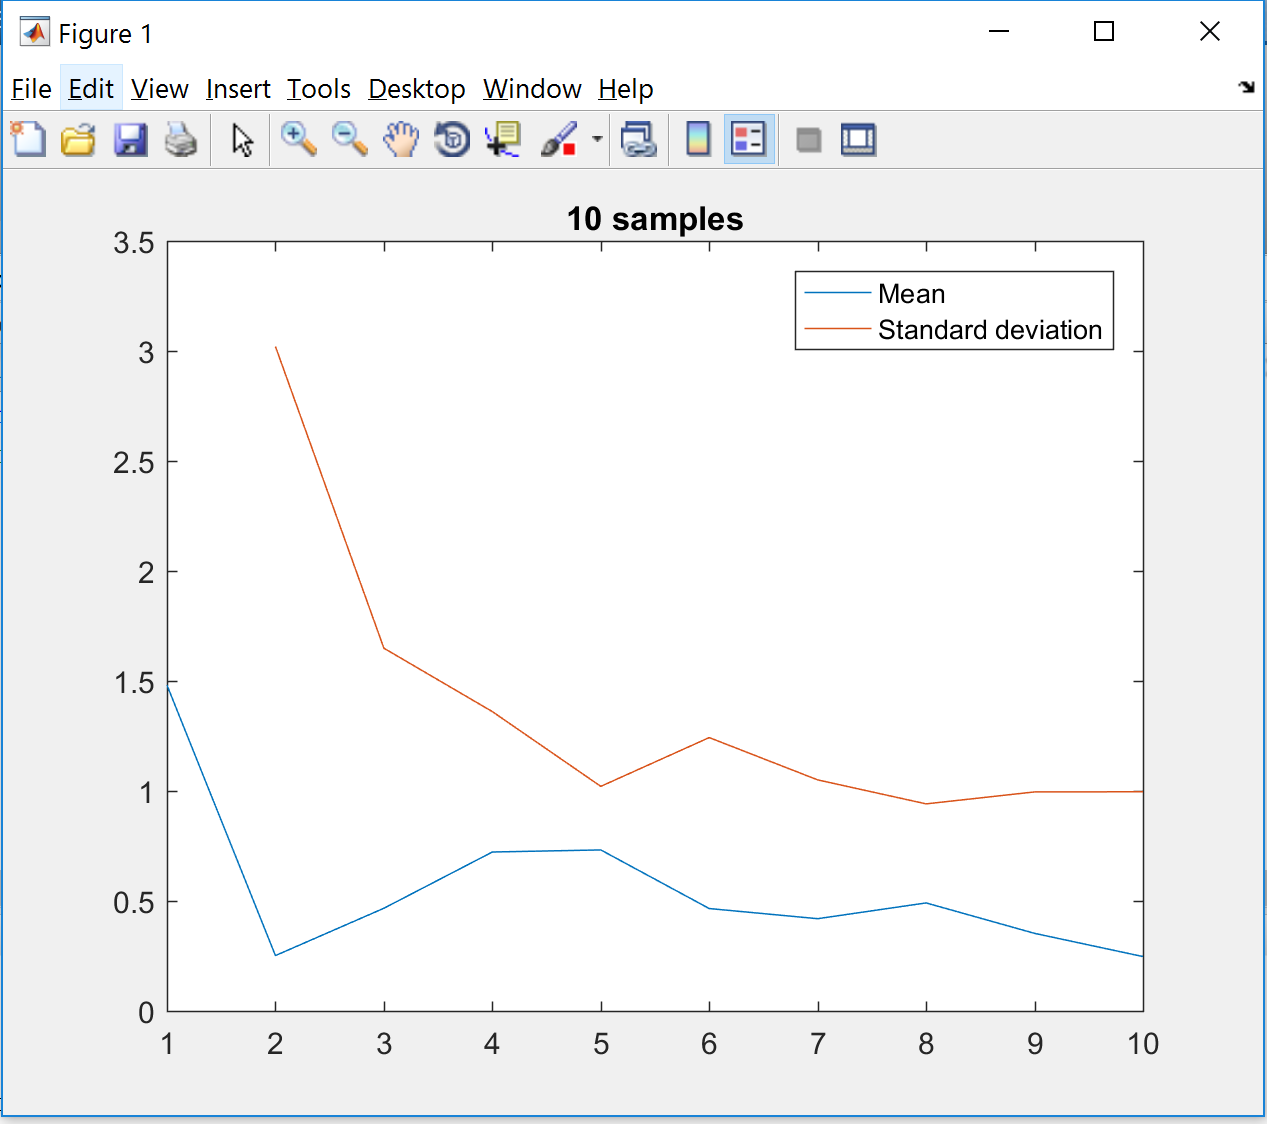
\includegraphics[width=100mm,scale=0.3]{5_1}\\
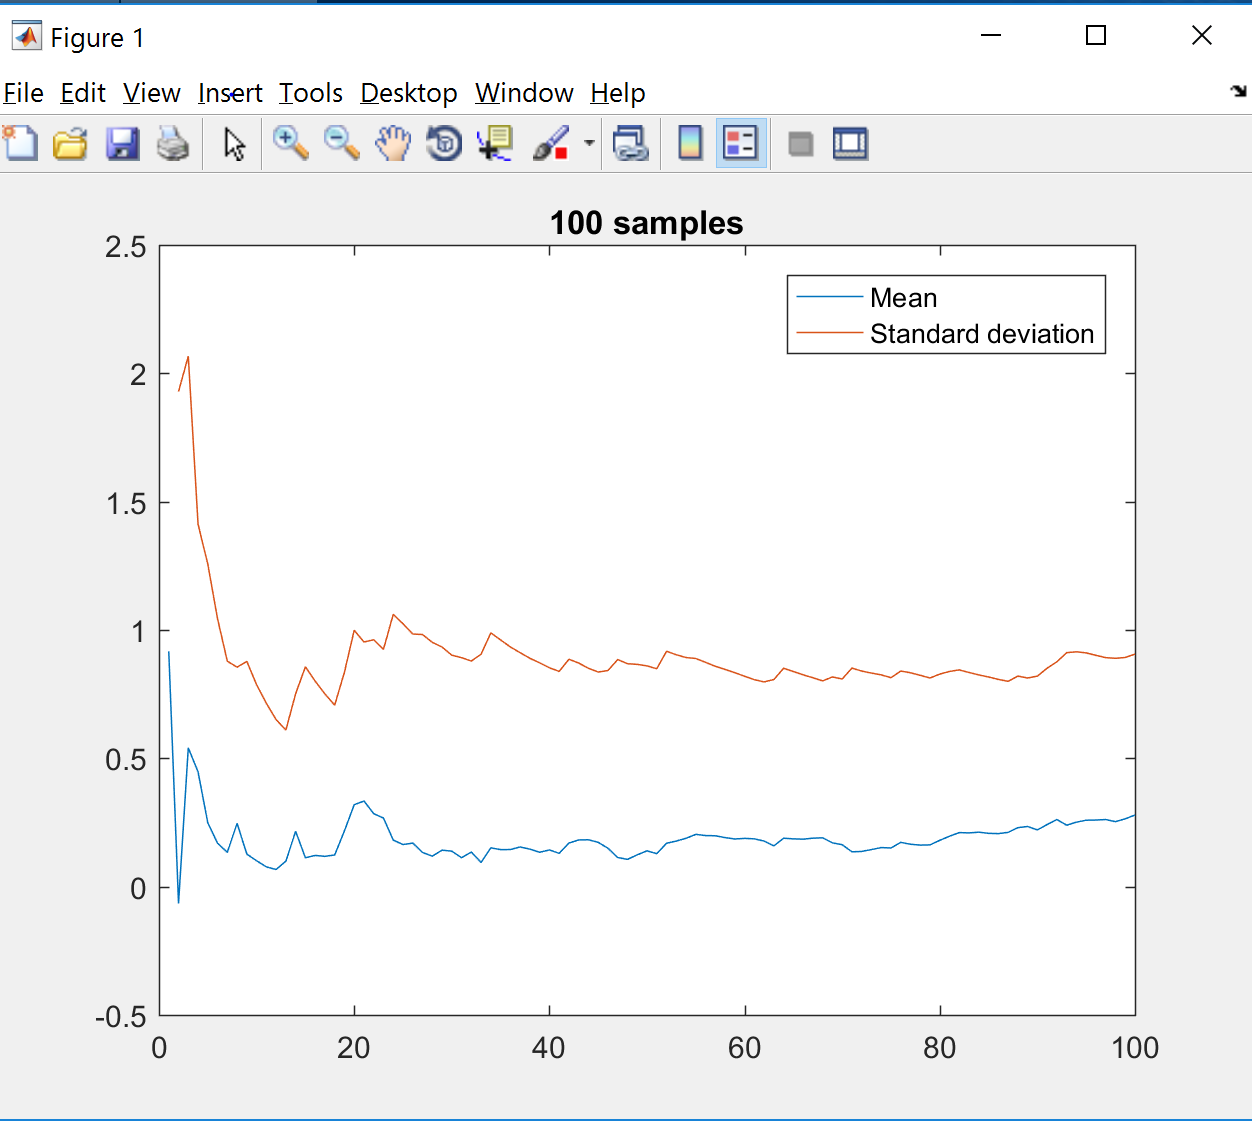
\includegraphics[width=100mm,scale=0.3]{5_2}\\
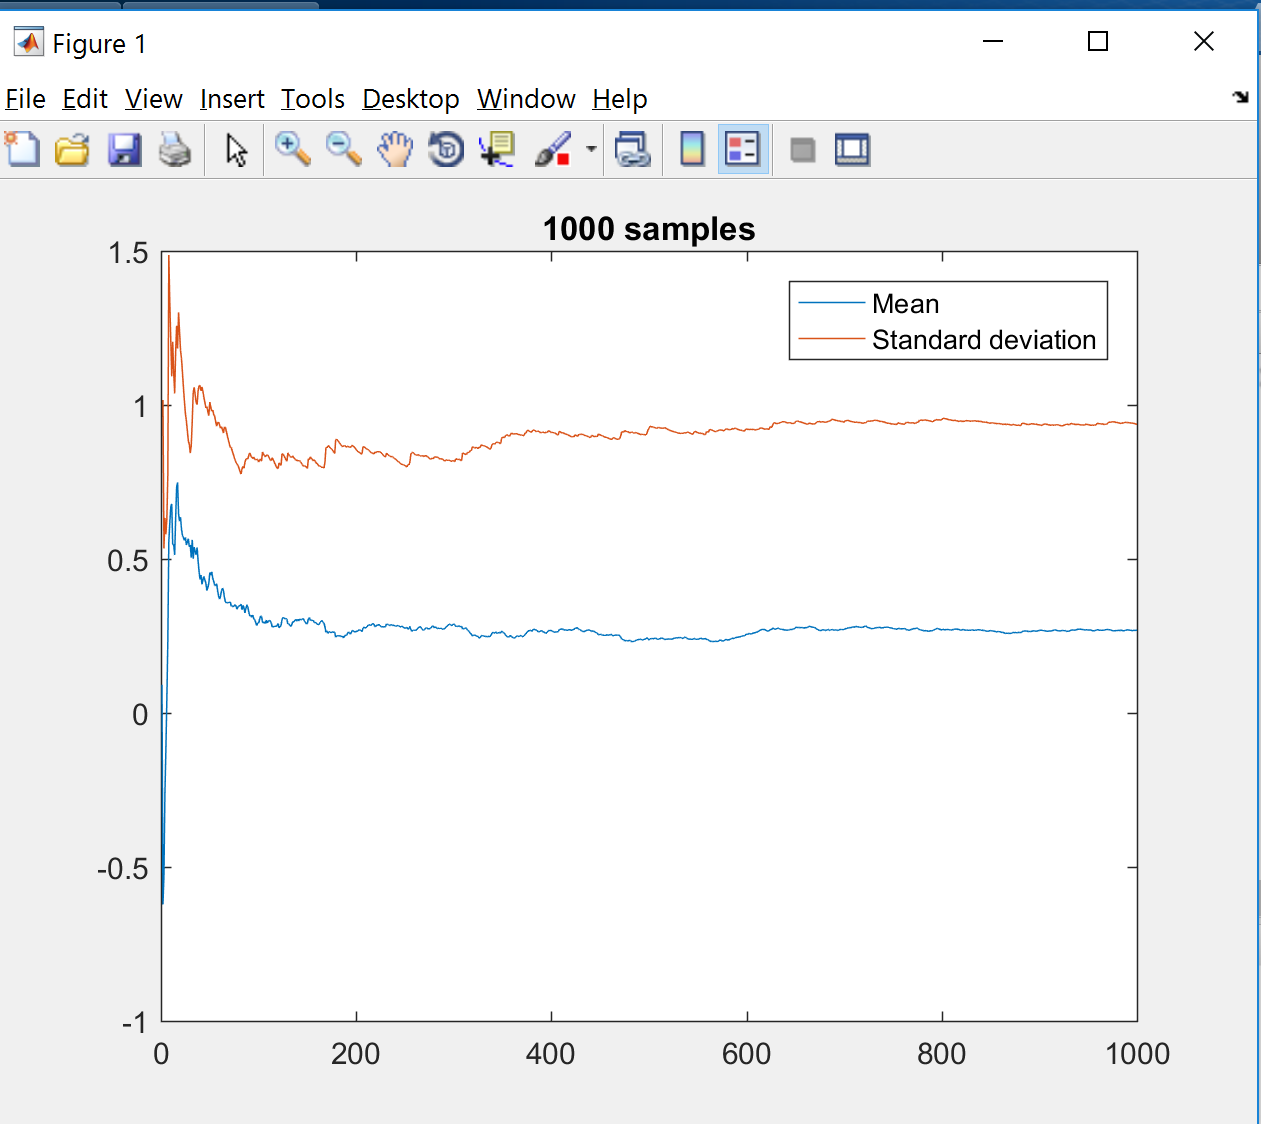
\includegraphics[width=100mm,scale=0.3]{5_3}\\
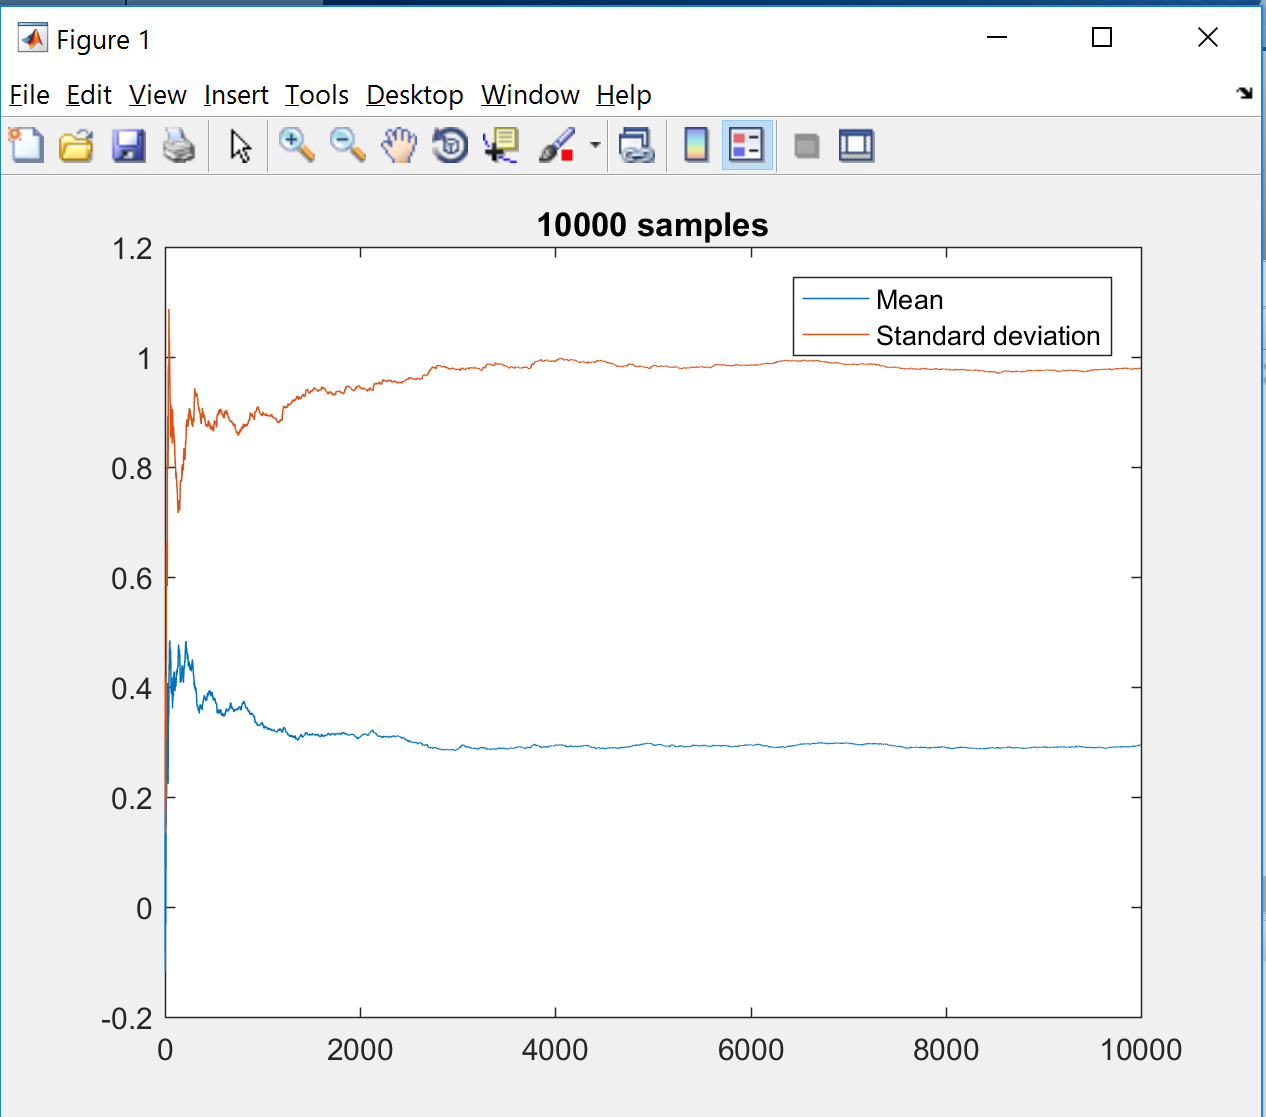
\includegraphics[width=100mm,scale=0.3]{5_4}\\
\begin{mdframed}[backgroundcolor=lightgray]
We see that as we increase the number of sample or data points from 10, 100, 1000 to 10000; the calculated mean and standard deviation converges to the actual mean, 0.3 and actual standard deviation, 1 of normal distribution. So we see that as the number of samples increases, it converges to actual mean and standard deviation quickly. I see that they are converging almost in $sqrt(n)$ speed.
\end{mdframed}
\end{itemize}

\section{(Agnostic) PAC Learning}

\subsection{Question 6}
Let $\fD$ be a distribution over $\fX \times \{0, 1\}$, and let $S = \{(\bx_1, y_1), \cdots ,(\bx_m, y_m)\}$ be a random sample from $\fD$. Let
\begin{align*}
\RiskD(h) &= \Pr_{(\bx,y)\sim \fD} [h(x) \neq y] \\
\RiskS(h) &= \frac{1}{m} |\{i: h(\bx_i)\neq y_i\}|
\end{align*}
Let $h_S$ and $h^*$ be the hypotheses in $\fF$ with minimum training and generalization error, respectively:
\begin{align*}
h_S = \argmin_{h \in \fF} \RiskS(h),\\
h^* = \argmin_{h \in \fF} \RiskD(h)~.
\end{align*}

Be sure to keep in mind that, unlike $h^*$, $h_S$ is a random variable that depends on the random sample $S$.
\begin{itemize}
\item Prove that
\[
\E[\RiskS(h_S)]\leq \RiskD(h^*) \leq \E[\RiskD(h_S)]~.
\]
\begin{mdframed}[backgroundcolor=lightgray]
We know that, by definition of Bayes Classifier,
$$ L_{D}(h^{*}) \leq L_D(h_S)$$
Taking expectation on both sides
$$ E[L_{D}(h^{*})] \leq E[L_D(h_S)]$$
Since $L_{D}(h^{*})$ is constant and we know that $E[constant] = constant$, we have
$$ L_{D}(h^{*}) \leq E[L_D(h_S)] \cdots 1$$
By definition of ERM, we know that
$$ h_S = \arg\,min_{h\in F}  L_S(h)$$
Thus,
$$L_{S}(h_{S}) = min_{h\in F}\ L_{S}(h)$$
In the above equation, we can consider h in the RHS to be any $h$ and $h^*$ is also one of those classifiers. Thus, we can rewrite the equation as,
$$L_{S}(h_{S}) \leq  L_{S}(h^*)$$
Again, taking expectation on both sides
$$E[L_{S}(h_{S})] \leq E[L_{S}(h^{*})] $$
We know that $E[L_{S}(h^*)] = L_{D}(h^*) $ Thus,
$$E[L_{S}(h_{S})] \leq  L_{D}(h^*) \cdots 2$$
From 1 and 2, we have proved
$$E[L_{S}(h_{S})] \leq L_{D}(h^{*}) \leq E[L_D(h_S)]$$
\end{mdframed}

\item We now make use of a stronger concentration inequality than the one used in class.
\begin{theorem}[McDiarmid’s inequality]
Let a function $f$ for which
\[
\forall x_1, \cdots, x_m, x_i' : |f(x_1,\cdots,x_i,\cdots,x_m)-f(x_1,\cdots,x'_i,\cdots,x_m)| \leq c_i,
\]
and $X_1,\cdots, X_m$ independent but not necessarily identically distributed random variables.
Then the following holds
\[
\Pr\left[\left|f(X_1, \cdots, X_m)- \E\left[f(X_1, \cdots, X_m)\right]\right|\geq\epsilon\right]\leq 2\exp\left(\frac{-2 \epsilon^2}{\sum_{i=1}^m c_i^2}\right)~.
\]
\end{theorem}
Using this theorem prove that, with probability at least $1-\delta$
\[
|\RiskS(f_S)-\E[\RiskS(f_S)]|\leq O\left(\sqrt{\frac{\ln(1/\delta)}{m}}\right),
\]
where there the constants hidden in the big-O notation do not depend on $|\fF|$.
\item Explain in words the meaning of what you proved and how we would expect training error to compare to test error when using a machine learning algorithm on actual data.
\end{itemize}

\subsection{Question 7}
Let $\fF$ a hypothesis class of binary classifiers. Show that if $\fF$ is agnostic PAC learnable, then $\fF$ is PAC learnable as well. Furthermore, if $A$ is a successful agnostic PAC learner for $\fF$, then $A$ is also a successful PAC learner for $\fF$
\begin{mdframed}[backgroundcolor=lightgray]
We need to show that with error $\epsilon$, the total loss is $L_D$ with probability $1-\delta$.
\[
P[L_D(f_x) lt \epsilon] > 1- \delta
\]
Agnostic PAC learnability says that, 
\[
P[L_D(f_s) - min_{f \in F} L_D(f) <= \epsilon] > 1-\delta
\]
Let us assume Bayes classifier is present in F.\\
So, $min_{f \in F} L_D(f) = 0$ means minimum loss among all classifiers in F becomes zero. Because, bayes classifier gives zero loss.
Now, the equation becomes 
\[
P[L_D(f_s) <= \epsilon]> 1 - \delta\\
\]
This shows that F is PAC learnable.\\

PartB\\
Now, we need to show that if A is a agnostic PAC learner for F then A is also a PAC learner for F.\\
A learner is a successful PAC learner when it successfully returns the hypothesis class with zero training error. That is it contains a Bayes classifier. Given that A is a successful agnostic PAC learner then  F returns a hypothesis with minimum training error. So, if F contains a Bayes classifier atleast one of the hypothesis has a zero training error. This means there exists atleast one hypothesis with least error. So, as A finds hypothesis with least error. This shows that A is a successful PAC learner.
\end{mdframed}

\section{Least Square Regression}

\subsection{Question 8}
Here you will code a Matlab (or Octave) function that implements the Least Square Regression algorithm. The input to the algorithm is the training set $S=\{(\bx_1,y_1), \cdots, (\bx_m,y_m)\}$, where $\bx_i \in \R^d$ and $y_i \in \R$, for $i=1, \cdots, m$. The output is the hyperplane solution of the Least Square problem, $\bw^*\in \R^d$. That is
\[
\min_{\bw,w_0} \sum_{i=1}^m (y_i -(w_0 + \langle \bw, \bx_i\rangle))^2
\]

\begin{itemize}
\item The prototype of the function must be 
\begin{verbatim}
[w,w_0] = train_ls(X,y,bias)
\end{verbatim}
where $X \in \R^{m \times d}$ is the matrix of $m$ input vectors in $d$ dimension, i.e. each input $\bx_i$ is a row of $X$, $y$ is a column vector of $m$ columns containing the labels associated to the training samples. The flag 'bias' signals if a bias $w_0$ must be used or not. If no bias is used, the returned value of $w_0$ is 0. The code must be robust to the case the the matrix $X^\top X$ is not invertible.

\begin{minted}[frame=single,framesep=10pt]{matlab}
function [w,w_0] = train_ls(X,y,bias)
% Handling bias. Appending column vector to matrix X.
if bias==1
    w_0 = 1;
    biasVec = ones(size(X,1), 1);
    X = [biasVec X];
else
    w_0 = 0;
end
%w = pinv(X) * y;
%w = sherman_morrison(X) *y;

% To handle non-invertible matrices. We calculate pseudoinverse from the
% formulae given in class.
X_sqr = transpose(X)*X;
if det(X_sqr) == 0
   v = diag(X);
      for i=1:length(v)
         if(v(i) ~= 0)
            v(i) = 1/v(i);
         else
             v(i) = 0;
         end
      end
      D = diag(v);
      V = orth(X_sqr);
      w = V*D*transpose(V)*transpose(X)*y;   
else
   w = inv(X_sqr) * transpose(X) * y;
end
\end{minted}

\item Implement another version, with prototype
\begin{verbatim}
w=incremental_train_ls(X,y)
\end{verbatim}
that construct the solution incrementally. This version does not have the bias $w_0$ term. This implementation must use the Sherman-Morrison formula to update the inverse of the matrix $X^\top X$:
\[
  (A + \bu\bv^\top)^{-1} = A^{-1} - \frac{A^{-1}\bu\bv^\top A^{-1}}{1 + \bv^\top A^{-1}\bu}
\]

Here we are calculating matrix inverse with Sherman-Morrison formulae.
\begin{minted}[frame=single,framesep=10pt]{matlab}
function [W] = incremental_train (X, y)
 
  [row, col] = size(X);
  W = [];

  X_New = X(1:100, 1:col);
  
  A = X_New' * X_New;
  Ainv = inv(A);
  
  for i = 101 : row
    v = X(i,:)';
    Ainv = Ainv - ((Ainv * (v * v') * Ainv) / (1 + (v' * Ainv * v)));
  end
  
  W = Ainv * transpose(X) * y;
end
\end{minted}

\item Verify numerically that the solutions of the two algorithms on a random training set are the same.
\begin{mdframed}[backgroundcolor=lightgray]
The Sherman-Mosrrison algorithm and general Matrix inverse algorithm are used to verify numerically if the results are same. The function is run on the same train data and got the output results as follows.
weights with Matrix inverse.
\[.0e+04 *
    (4.5193,
    0.1800,
   -0.0015,
    0.0074,
   -0.0045,
    0.0154,
   -0.7804,
   -0.2051)
 \] 
weights with Sherman-Mosrrison algorithm, i.e. using incremental training algorithm.
\[
1.0e+04 *
    (4.5193,
    0.1800,
   -0.0015,
    0.0074,
   -0.0045,
    0.0154,
   -0.7804,
   -0.2051)
\]
\end{mdframed}
   
\item Discuss the computational complexity of both versions and compare them.
\begin{mdframed}[backgroundcolor=lightgray]
According to Sherman-Morrison formula,
We append row vectors incrementally with u and v. So, we see that there is one rank change in the matrix resulting in one rank change in the inverse of that matrix.
Also, we see that inverse of matrix is computed in $n^2$ operations whereas the regular matrix matrix inverse computation requires $n^3$ operations.
\end{mdframed}
\end{itemize}


\subsection{Question 9}
In this question, you are supposed to implement linear regression using polynomial basis functions. Use only monomials of a single variable, e.g. $(x_1, x_1^2, x_1^3, \cdots, x_2, x_2^2, \cdots)$, and no cross-terms, e.g. $(x_1 x_2, x_1^2 x_2, \cdots)$.
\begin{itemize}
\item Implement a Matlab function that normalizes all the input data attributes to be between -1 and 1.
\begin{verbatim}
[X_train_norm, X_test_norm] = normalizeAll(X_train, X_test)
\end{verbatim}
Note that only training data can be used for learning the normalization transformation. This will be used to prevent numerical instability in dealing with numbers that are too big or too small.

\begin{minted}[frame=single,framesep=10pt]{matlab}
% [X_train_norm, X_test_norm] = normalizeAll(X_train, X_test)
function [X_train_norm, X_test_norm] = normalizeAll(X_train, X_test)
    % X_train is a MXD matrix, 
    % it means M data points in D dimensional space.

    X_train_norm = -1 + 2.*(X_train - min(X_train))./(max(X_train) - min(X_train));
    X_test_norm = -1 + 2.*(X_test - min(X_test))./(max(X_test) - min(X_test));
end
\end{minted}

\item Implement a function that generates a matrix of input samples that contains the powers of each feature from 1 to $k$
\begin{verbatim}
[X_poly] = generate_poly_features(X,k)
\end{verbatim}

\begin{minted}[frame=single,framesep=10pt]{matlab}
% concatenate all the degree polynomials to form X_poly
function [X_poly] = generate_poly_features(X,k)
    X_poly = X;
    for i = 2:k
        X_poly = horzcat(X_poly, X.^i);
    end
end
\end{minted}

\item Use the training and test data provided in the file ``cadata.mat''. They correspond to a random split train/test of the Housing dataset from the UCI repository. The task is to predict the median house value from features describing a town.
Use the code you wrote above to generate polynomial features from $k=1$ to $k=5$, normalize the features, and train 5 different LS regressors (with bias $w_0$) with these features. Plot training error and test error for each value of $k$ and discuss the results.

\begin{minted}[frame=single,framesep=10pt]{matlab}
function polynomialRegression(X_train, y_train, X_test, y_test)
    %train error vector for each degree of polynomial.
    rmseTrain = zeros(5, 1);
    %test error vector for each degree of polynomial.
    rmseTest = zeros(5, 1);
    
    %iterating over each degree of polynomial
    for i = 1:5
        %generate polynomial features for train and test sample
        train = generate_poly_features(X_train, i);
        test = generate_poly_features(X_test, i);
        
        %normalize train and test sample
        [A, B] = normalizeAll(train, test);
        [w, w_0] = train_ls(A, y_train, 1);
        
        %Append a column vector in case of bias
        if(w_0 == 1)
            A = [ones(size(A,1),1) A];
            B = [ones(size(B,1),1) B];
        end    
        
        %Finally calculate the least square error
        rmseTrain(i,:) = mean((y_train - A*w).^2);
        rmseTest(i,:) = mean((y_test - B*w).^2);
    end

    % plot the least square error for train and test samples.
    plot(rmseTrain);hold on;
    plot(rmseTest);
    xlabel('Degree of the polynomial');
    ylabel('RMSE');
    legend('training error', 'test error');
end    
\end{minted}
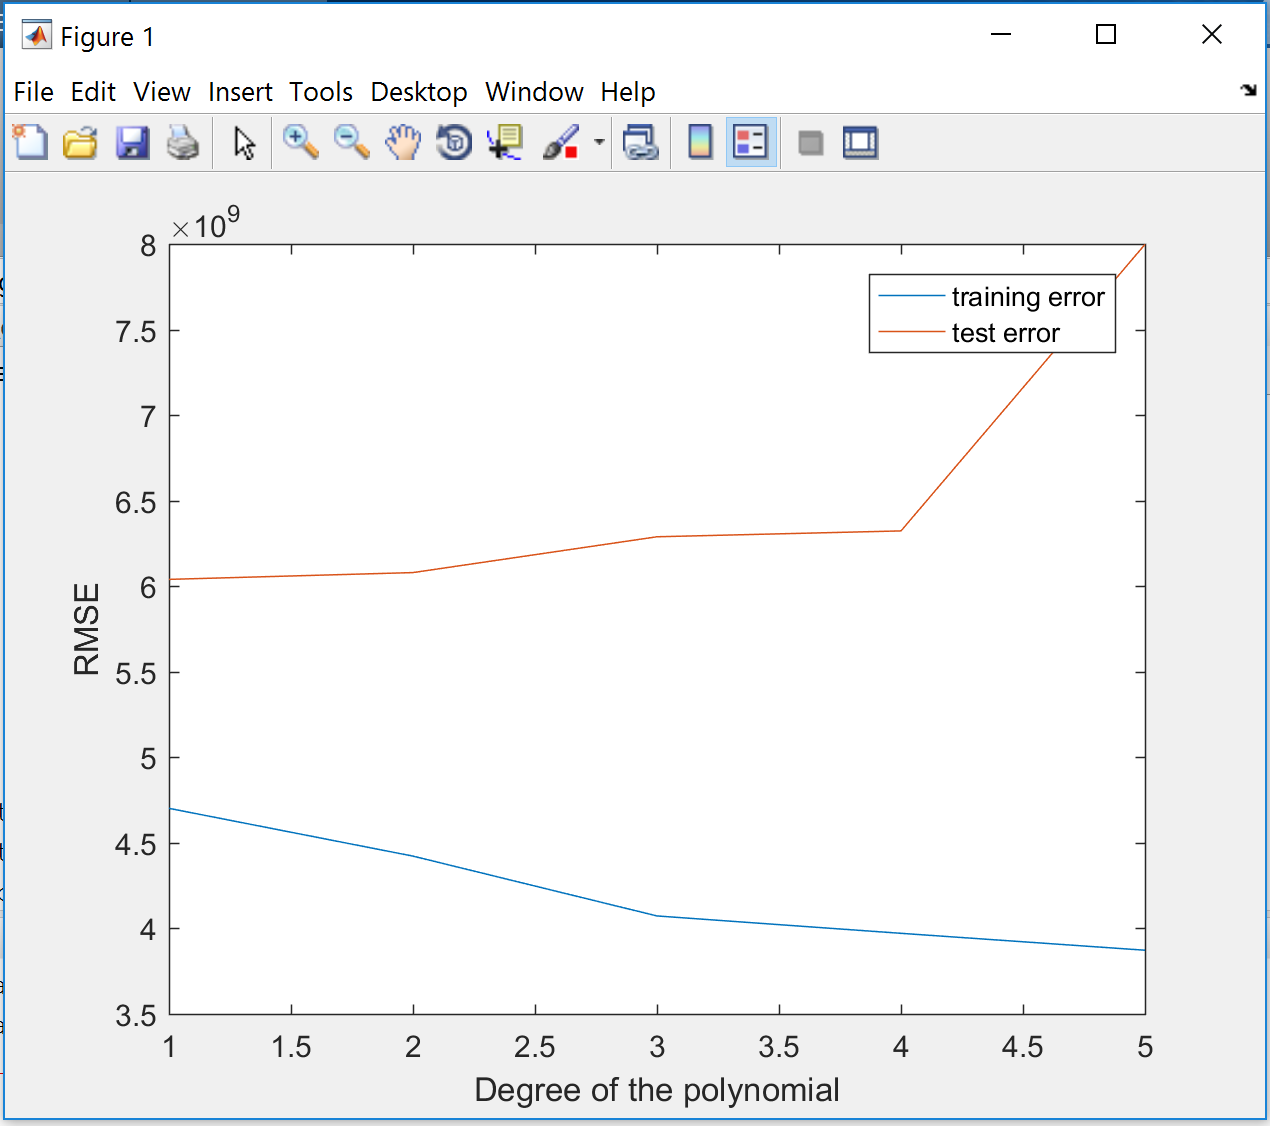
\includegraphics{9_1}\\
Training error and test error for each polynomial of degree value k from 1 to 5 are plotted. We can see that as the degree of polynomial increases, the training error decreases as it tend to fit the data more appropriately. But in case of test samples, as the degree of polynomial increases, the test error remains the same but after degree 4, when the degree of polynomial increases, the test error suddenly increases exponentially. This is because the test samples do not fit the distribution generated by train data and with every new sample from test set, the error starts to increase. \\
In summary as the degree of polynomial increases, the distribution generated becomes biased to training samples and tends to over-fit the data. So, test error starts to increase exponentially after a threshold polynomial degree.
\end{itemize}
\end{document} 